

\documentclass[10pt, conference, compsocconf]{IEEEtran}

\usepackage{graphicx}
\usepackage{algorithmic,listings}
\lstset{language=C,basicstyle=\small\ttfamily, basewidth=0.51em}
\usepackage{url}
\usepackage{tabularx}
\usepackage{subfig}
\usepackage{float}
\usepackage{underscore}
% correct bad hyphenation here
\hyphenation{op-tical net-works semi-conduc-tor}

\graphicspath{{figures/}}
\pagestyle{plain}
\begin{document}


\title{Application-Level Regression Testing Framework using Jenkins}


% author names and affiliations
% use a multiple column layout for up to two different
% affiliations


% conference papers do not typically use \thanks and this command
% is locked out in conference mode. If really needed, such as for
% the acknowledgment of grants, issue a \IEEEoverridecommandlockouts
% after \documentclass

% for over three affiliations, or if they all won't fit within the width
% of the page, use this alternative format:
%
\author{\IEEEauthorblockN{Timothy Bouvet, Reuben Budiardja, Galen Arnold}
%xxxx\IEEEauthorrefmark{3} and
%xxxx\IEEEauthorrefmark{4}}
%\IEEEauthorblockA{\IEEEauthorrefmark{1}National Institute for Computational Science\\
National Center for Supercomputing Applications\\
University of Illinois at Urbana-Champaign, 61801\\
National Institute for Computational Sciences\\
The University of Tennessee, Knoxville, TN 37996\\
\{tbouvet@illinois.edu,reubendb@utk.edu,gwarnold@illinois.edu\}}
%\IEEEauthorblockA{\IEEEauthorrefmark{4}Electrical Engineering and Computer Science Department\\University of Tennessee, Knoxville, TN 37996\\xx@eecs.utk.edu}
%}


% use for special paper notices
%\IEEEspecialpapernotice{(Invited Paper)}



% make the title area
\maketitle
\thispagestyle{plain}

\begin{abstract}
This paper will explore the challenges of regression testing and monitoring of large scale systems such as NCSA’s Blue Waters. Our goal was to come up with an automated solution for running user-level regression tests to evaluate system usability and performance. Another requirement was to find an automated solution for running a suite of test jobs that reveal the system health after upgrades and outages before returning the system to service. We evaluated test frameworks such as Inca [1] and Jenkins [2]. Jenkins was chosen for its versatility, large user base, and multitude of plugins including plotting test results over time. We utilize these plots to track trends and alert us to system-level issues before they are reported by our partners (users). Not only does Jenkins have the ability to store historical data but it can also send customized notifications (e.g. send email or text pages) based on the result of a test. Some of the requirements we had include two-factor authentication to access Jenkins GUI with privileges to execute tests and account management through LDAP. In this paper we describe our implementation of these requirements to ensure a secure and usable deployment of a Jenkins instance.

Our Jenkins instance was deployed on a vSphere managed VM running Centos 6.8. Security was of the highest concern since Jenkins has the ability to execute commands on our login nodes. Jenkins is set to log in as a standard user account with password-less access (commands to the login nodes can be input via Jenkins GUI) using ssh keys scoped to the VM. The VM (bwjenkins) was closely vetted by our security team on our test and development system (TDS) before it was allowed access to Blue Waters. Iptables was used to lock bwjenkins down to a small internal ip space to ensure the highest security. An anonymous user account was enabled with ‘read-only’ access to view current and historical test results. During a test, Jenkins downloads software, builds the software, submits a job, awaits completion, gathers and plots the results or returns error information during a failure. These are full end to end functionality tests of the programming environment, queueing system, license servers and they provide historical metrics to quickly detect regressions.

In this paper we describe in detail our challenges and experiences in deploying Jenkins as a user-level system-wide regression testing and monitoring framework for Blue Waters. We will also show some application-based system-level tests we have implemented in Jenkins and share results of those tests. The deployment of Jenkins allows us to monitor and detect issues as early as possible from the perspective of a user on Blue Waters, eventually providing a more efficient service for better user experience.
\end{abstract}

\begin{IEEEkeywords}
Performance; Benchmarking; Computer architecture
\end{IEEEkeywords}


% For peer review papers, you can put extra information on the cover
% page as needed:
% \ifCLASSOPTIONpeerreview
% \begin{center} \bfseries EDICS Category: 3-BBND \end{center}
% \fi
%
% For peerreview papers, this IEEEtran command inserts a page break and
% creates the second title. It will be ignored for other modes.
\IEEEpeerreviewmaketitle

\section{Motivation}
Our goal was to come up with an automated solution for running user-level regression tests to evaluate system usability and performance. Another requirement was to find an automated solution for running a suite of test jobs that reveal the system health after upgrades and outages before returning the system to service.
\section{Jenkins Configuration}
\label{sec:JenkinsConfiguration}

\subsection{Introduction to Jenkins}
Jenkins [2] is a self-contained, open source automation server which can be used to automate all sorts of tasks such as building, testing, and deploying software. Jenkins can be installed through native system packages, Docker, or even run standalone by any machine with the Java Runtime Environment installed. 
To install from rpm as root:
wget -O /etc/yum.repos.d/jenkins.repo http://pkg.jenkins-ci.org/redhat/jenkins.repo
rpm --import https://jenkins-ci.org/redhat/jenkins-ci.org.key
yum install jenkins
\subsection{Master-Node Configuration}
We added a standard user account to our cluster that will execute the Jenkins tests. Unique ssh keys were generated on the Jenkins Server for accessing the user account on production and test environments.  The keys on the server are located in Jenkins home directory (/var/lib/jenkins/.ssh). Using the GUI management console, the keyfile location and passphrase was entered under Manage Jenkins, Configure System, SSH remote hosts section. A unique SSH site is configured for our TDS, production and development login nodes.   

\subsection{Accessing Login Nodes}
The ssh public key generated on Jenkins Server was deployed in the login node user account. The login node sshd_config was modified to allow Public Key Authentication from the Jenkins Server IP.     


\section{Authentication and Authorization}
\label{sec:AuthenticationAuthorization}

\subsection{Security Considerations}
Enabling Jenkins access to Blue Waters posed some unique security hurdles that we had to overcome. Blue Waters is an OTP only restricted access system. Jenkins has the ability to execute user-level commands on our login nodes. Jenkins has some unfortunate default settings. The access control is set to "Jenkins' own user database," and the "Allow users to sign up" option is enabled, so if you don't have an account, you can create one by providing your name, e-mail and a password. Additionally, there's an authorization option enabled which says "Logged-in users can do anything." So, once you complete the sign up form, you have full admin access to the system.  This required us initially to test the deployment with our test and development (TDS) CRAY. This resulted in the following requirements. Restricted OTP access to the physical system that will host Jenkins. In addition, OTP only access to the Jenkins GUI command console that must be contained within our IP space.  The Jenkins GUI will also restrict the command console access to our Blue Waters LDAP server. 

\subsection{Configuration Choices}
Jenkins instance was deployed on a vSphere managed VM running Centos 6.8. The VM allows restricted host-based ssh access from two secure OTP only administrative systems. The Jenkins GUI presented additional challenges. The Jenkins GUI is configured to log in as a standard user account with pass-wordless access (commands to the login nodes can be input via Jenkins GUI) using ssh keys scoped to the VM. We restricting access to the physical VM (bwjenkins) and the Jenkins GUI utilizing iptables, SSL and OTP.  A reverse proxy was used to run Jenkins behind apache/http with SSL for access to the administrative console. All the configuration is in /etc/httpd/conf.d/ssl.conf. Anonymous access to the Jenkins GUI was allowed for limited read only view of test status and historical plots. The Anonymous access view is not restricted. \\
(config file snippets below)

\begin{lstlisting}
/etc/ssh/sshd_config:
Match Host bwbh1.ncsa.illinois.edu,
bwbh2.ncsa.illinois.edu
HostbasedAuthentication yes

/etc/sysconfig/iptables:
-A INPUT -s 141.142.0.0/16 -m state --state NEW -m tcp 
-p tcp --dport 22 -j ACCEPT
-A INPUT -s 172.16.0.0/15 -m state --state NEW -m tcp 
-p tcp --dport 22 -j ACCEPT *delete maybe*
-A INPUT  -m state --state NEW -m tcp -p tcp --dport 80 
-j ACCEPT
-A INPUT -s 141.142.0.0/16 -m state --state NEW -m tcp 
-p tcp --dport 443 -j ACCEPT

/etc/httpd/conf.d/ssl.conf:
Listen 443
<VirtualHost _default_:443>
SSLSessionCache         shmcb:/var/cache/mod_ssl/scache
SSLSessionCacheTimeout  300
ServerName bwjenkins.ncsa.illinois.edu:443
 # -- The following sets ReverseProxy for Jenkins
  ProxyRequests       Off
  ProxyPreserveHost   On
  AllowEncodedSlashes On
  <Proxy *>
    Order deny,allow
    Allow from all
  </Proxy>
  ProxyPass       / http://localhost:8080/ nocanon
  ProxyPassReverse / http://localhost:8080/
  ProxyPassReverse / http://bwjenkins.ncsa.illinois.edu/
  RequestHeader set X-Forwarded-Proto "https"
  RequestHeader set X-Forwarded-Port "443"

  DefineExternalAuth pwauth+session pipe /usr/local/bin/
  pwauth+session
  <LocationMatch / > 
    AuthType Basic
    AuthBasicProvider external
    AuthName "NCSA RSA OTP login" 
    AuthExternal pwauth+session
    require valid-user
    
    RequestHeader unset "X-Forwarded-User"
    RequestHeader set "X-Forwarded-User" (REMOTE_USER)

  </LocationMatch>
\end{lstlisting}

\subsection{LDAP with Jenkins}
\begin{figure}[H]
\centering
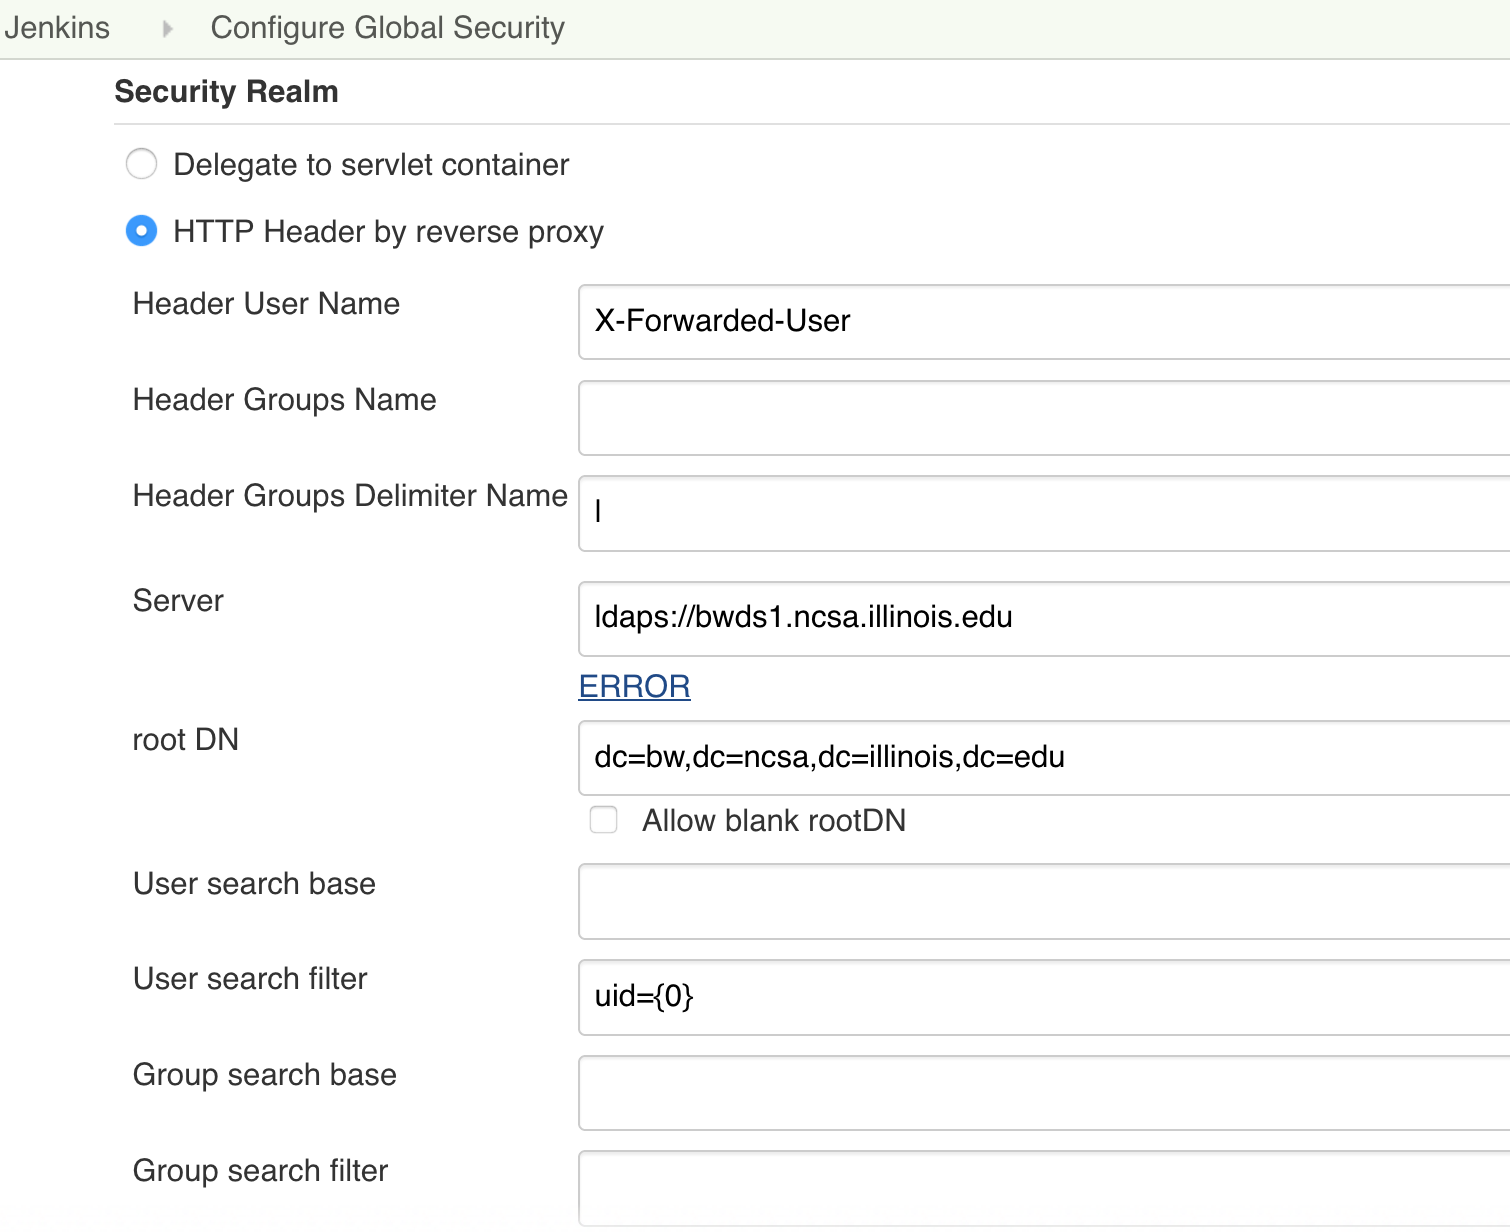
\includegraphics[width=0.5\textwidth]{LDAP-Jenkins}
\caption{ Use LDAP with Jenkins }
\label{fig:LDAP-Jenkins}
\end{figure}
To enable LDAP, the LDAP Plugin was installed. To configure, from the console view, select Manage Jenkins, select Configure Global Security. In the Security Realm section select the Advanced... tab. Input your LDAP server name and root DN. Click the Test Button.\\
\\
My first stab at this failed as an anonymous connection to our LDAP because we are using a local CA.
WARNING: Failed to search LDAP for username, 
sun.security.provider.certpath.SunCertPathBuilderException:
unable to find valid certification path to requested target\\
\\
We had to add our certificate to the keystore:
/usr/java/default/jre/bin/keytool -list -keystore cacerts -imle /etc/openldap/cacerts/cacert.pem
Enter keystore password: Trust this certificate? [no]:  yes\\
Certificate was added to keystore

\subsection{Configure Global Security}
\begin{figure}[H]
\centering
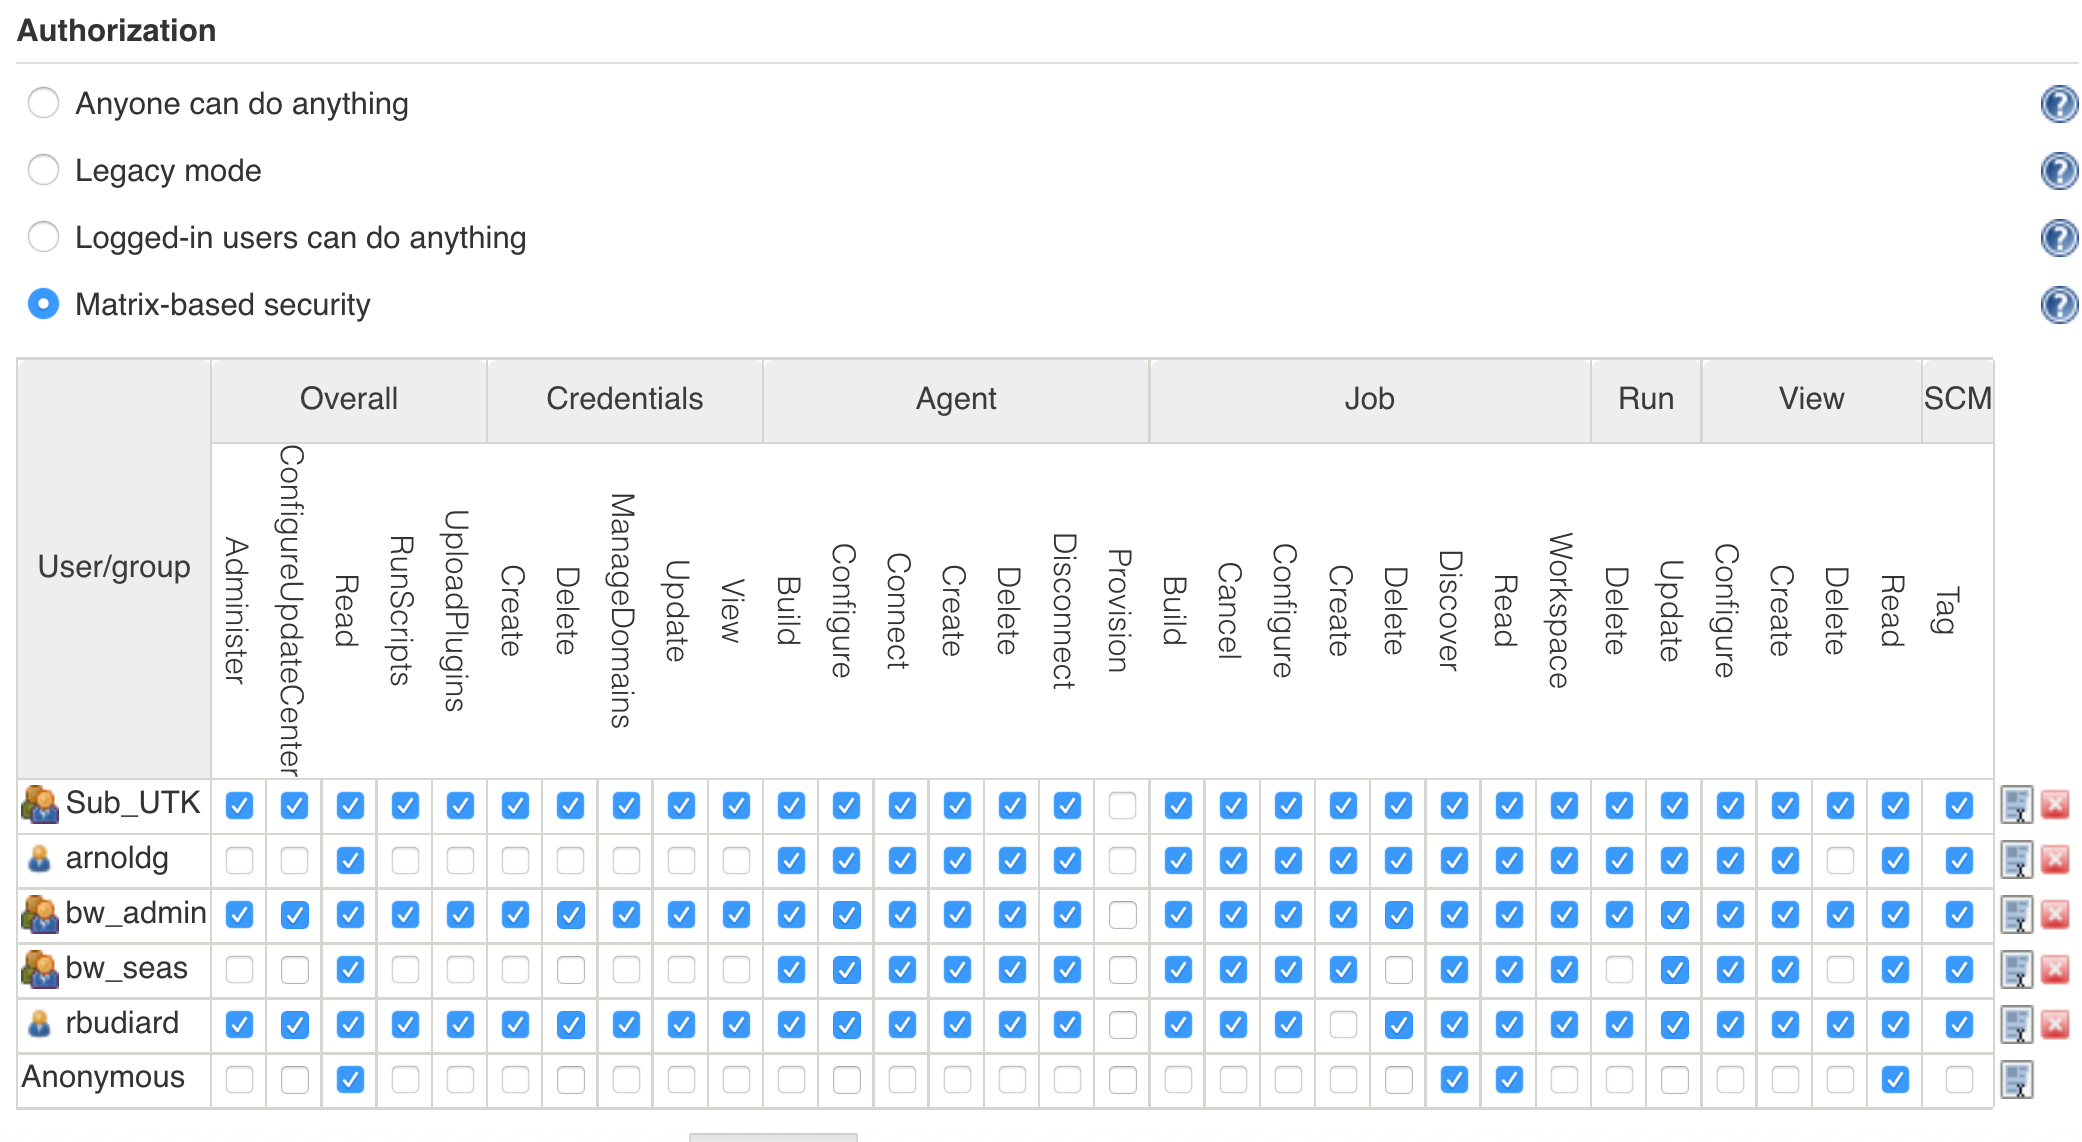
\includegraphics[width=0.5\textwidth]{Configure-Global-Security}
\caption{ Configure Global Security }
\label{fig:Configure-Global-Security}
\end{figure}
We are allowing access by username and LDAP groups. The permissions can be scoped for individuals and groups. An example is removing Job delete permissions to prevent one user or group from deleting each other's jobs. 

\section{Anatomy of A Test}
\label{sec:TestAnatomy}
New software projects are required to be tested on our TDS and approved before deployment on Blue Waters and this is one of our key best practices.  Once a test is deployed it is assigned to a specific Jenkins tab via the "Edit View" link associated with that tab.  Tests still in development reside in the "All" tab view until they have been peer reviewed by at least one other test developer.
\subsection{test description}
We require a description for each test to describe: what is tested, resources used by the test, intent of the test, and scheduling frequency.
\subsection{limits log files}
The Jenkins test VM filled to capacity after the first few weeks of intensive use and an influx of several new tests that output long source code build detail.  We retroactively modified all tests to limit the number of old build logs retained (max 50 for most tests). 
\subsection{ssh to a login host}
There are several target ssh hosts which may be selected from our instance: the test rack JYC, the main system, and the new software deployment login node within the main system.  None of our tests run locally within the Jenkins VM.
\subsection{run shell commands}
A test is composed of shell command and where possible we try to be as transparent with our test construction as possible.  We prefer commands in the Jenkins configuration over running a script in the filesystem on the remote ssh target.  Scripts that are remote run with verbose mode or are displayed via "cat -n" to save output to the Jenkins console log and make for simpler debugging when a test fails.
\subsubsection{test completes on login node}
Some tests run only on the ssh login node and return more or less immediately.  Examples include tests for batch system functionality, ssh functionality, and filesystem functionality.  These tests are very similar in style to unit tests which target a limited set of functionality.
\subsubsection{test is submitted to batch system}
More comprehensive tests typically build and run an application or benchmark through the batch system.  These tests exercise multiple aspects of the system: (filesystem, compilers and modules, high-speed network, external connectivity to the internet...).  They block to completion so that we do not overburden the batch system with tests.  Unlike tests that run entirely on a login node, completion time can be highly variable depending on the queue depth and available backfill windows for the batch system.
\subsection{post test actions}
\subsubsection{scp files back to Jenkins host}
Most comprehensive tests produce output that we use when debugging a failed test.  They may also produce plot data.  These files are copied back to the Jenkins host so that they can be viewed and/or incorporated into the plot feature of Jenkins.
\subsubsection{plots}
Successful tests save plot files and contribute a new data point to a plot.  The Jenkins server accumulates the data as rows in a spreadsheet (under /var/lib/jenkins/jobs/ ) and plots them via the "Plots" link for a test.
\subsection{email notification}
When the state of a test changes, email notification is sent to the test owner.  As a best practice we also use the email notification as a method of tracking authorship and each test has an email owner even if notifications are disabled for the test.


\section{SWTools Integration}
\label{sec:SWToolsIntegration}
\subsection{SWTools with Jenkins}
\begin{figure}[H]
\centering
\includegraphics[width=0.5\textwidth]{swtools-Jenkins}
\caption{ Use SWTools with Jenkins }
\label{fig:swtools-jenkins}
\end{figure}

\subsection{SWTools with Lammps}
\begin{figure}[H]
\centering
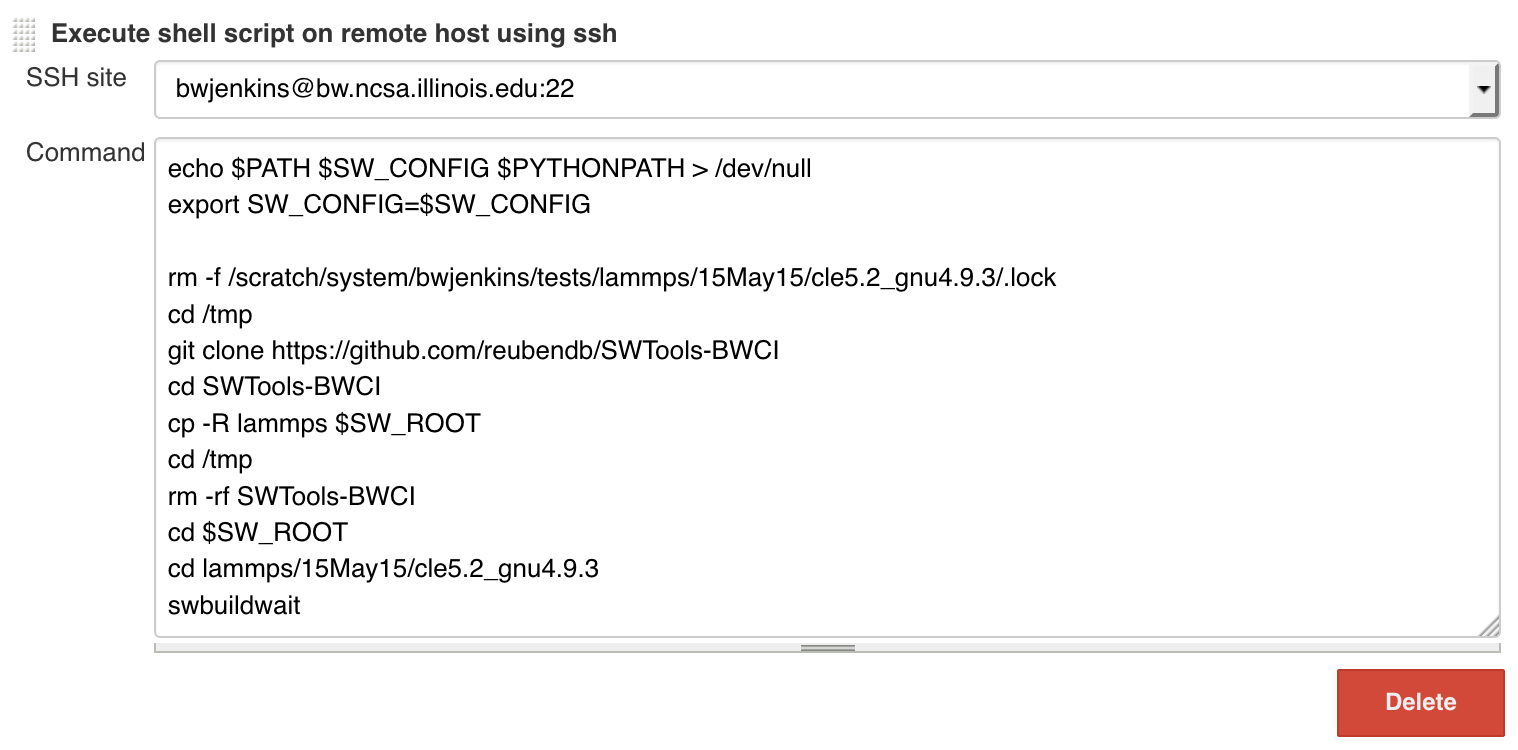
\includegraphics[width=0.5\textwidth]{swtools-lammps}
\caption{ SWTools with Lammps }
\label{fig:swtools-lammps}
\end{figure}

\section{Use Cases}
\label{sec:results}
\subsection{IOR Lustre scratch test}
We created Jenkins tests to periodically run the IOR MPI parallel i/o benchmark at modest scale and validate filesystem functionality and performance for the scratch filesystem. The test is scaled to provide representative performance numbers for a typical small application while not creating performance issues with other jobs or the larger filesystem.  One of our best practices is to provide a management level summary description for casual jenkins users who want to view the tests but do not need to understand the full Jenkins configuration and execution details.  
\begin{figure}[H]
\centering
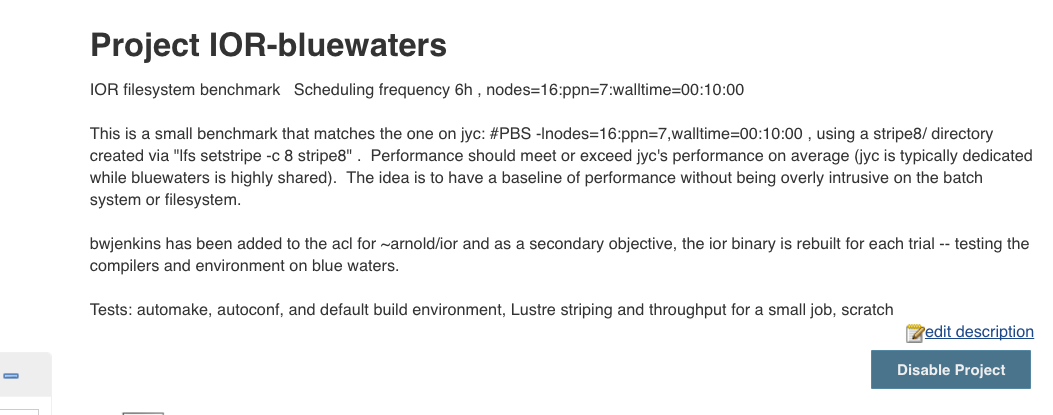
\includegraphics[width=0.5\textwidth]{IOR-bluewaters-descr}
\caption{ IOR description in jenkins }
\label{fig:IOR-bluewaters-descr}
\end{figure}
Where possible, tests build from source and exercise multiple user-facing system components such as: git for external connectivity and modules to test defaults in the environment.  Where scripts on the remote SSH site are used, they are echoed and/or displayed with "cat -n" to make console output verbose and easy to debug in case of errors.  
\begin{figure}[H]
\centering
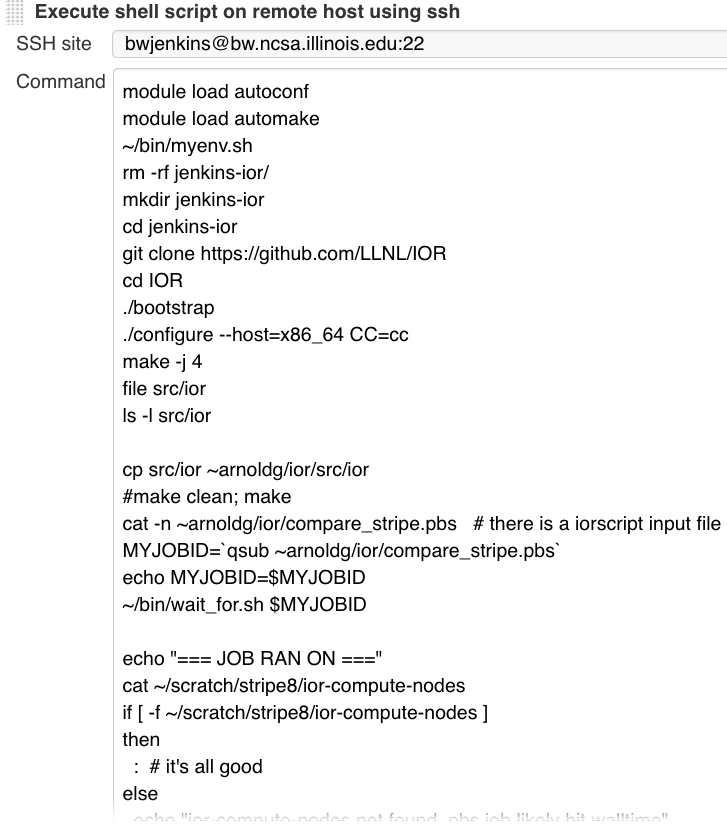
\includegraphics[width=0.5\textwidth]{IOR-configuration-sample}
\caption{ IOR configuration sample }
\label{fig:IOR-configuration-sample}
\end{figure}
The IOR test is set to run as scheduled by Jenkins with a best-effort through our batch system.  The test synchronously blocks such that the next test will not start until the previous one has completed.  We employ a watchdog script to monitor the batch queue and keep the test active until the system marks it as finished.  This has the side effect of making the minimum test time an integer multiple of the sleep time in the watchdog script.  This may be adjusted to fit individual site needs.
\begin{lstlisting}[frame=tb,captionpos=t,language=bash,caption={pbs/torque watchdog script}, label=lst:watchdog]
#!/bin/bash
echo "=== RUNNING $0 ==="
if [ $# -lt 1 ]
then
  echo "$0: missing argument for jobid"
  exit 1
fi
while true
do
	MYQSTAT=`qstat $1`
	if test "$MYQSTAT" = ""
        then
		echo $1 finished
		exit
	else
		DATE=`date`
		echo "$DATE: waiting for $1 to finish"
	fi
	sleep 5m
done
\end{lstlisting}

\begin{figure}[H]
\centering
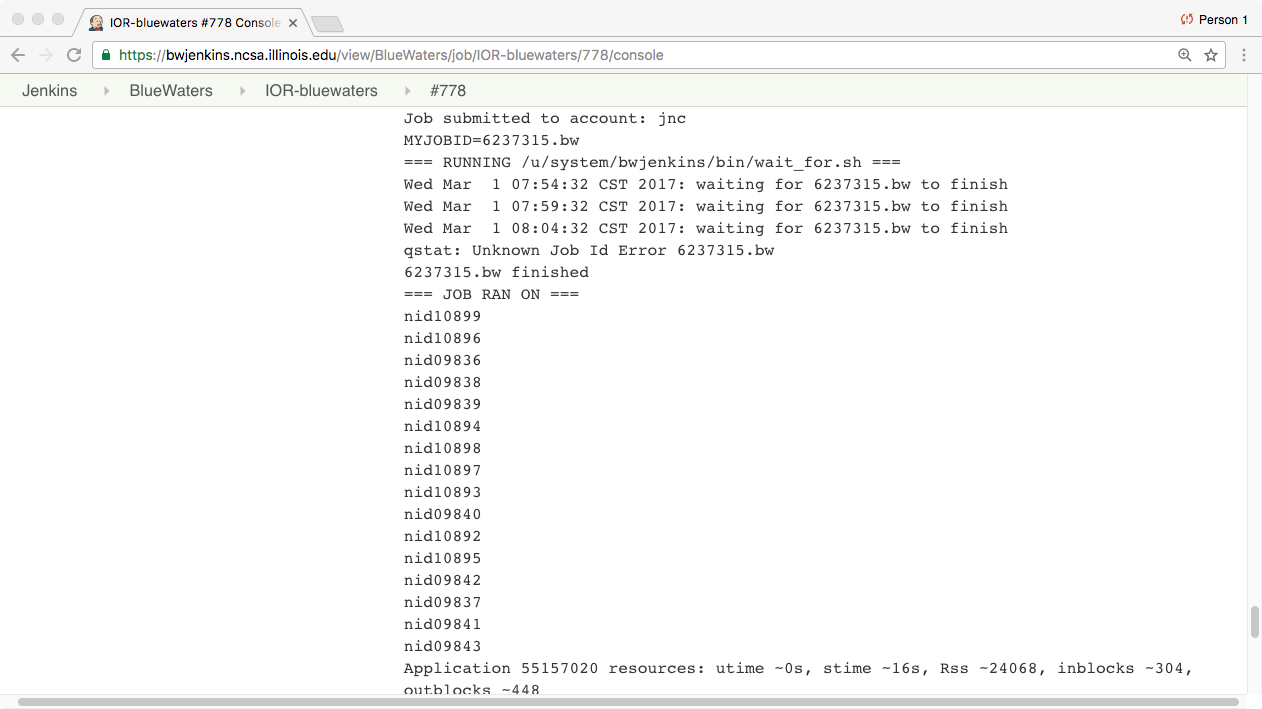
\includegraphics[width=0.5\textwidth]{IOR-watchdog-out}
\caption{ IOR watchdog console output }
\label{fig:IOR-watchdog-out}
\end{figure}
For tests that produce an interesting performance metric like IOR, we save that output to the file format expected by Jenkins and use plotting feature to produce plots. 
\begin{lstlisting}[frame=tb,captionpos=t,language=bash,caption={sample YVALUE output file}, label=lst:yvalue]
bwjenkins$ cat myiorREADnumber.dat 
YVALUE=8352.71
\end{lstlisting}
\begin{figure}[H]
\centering
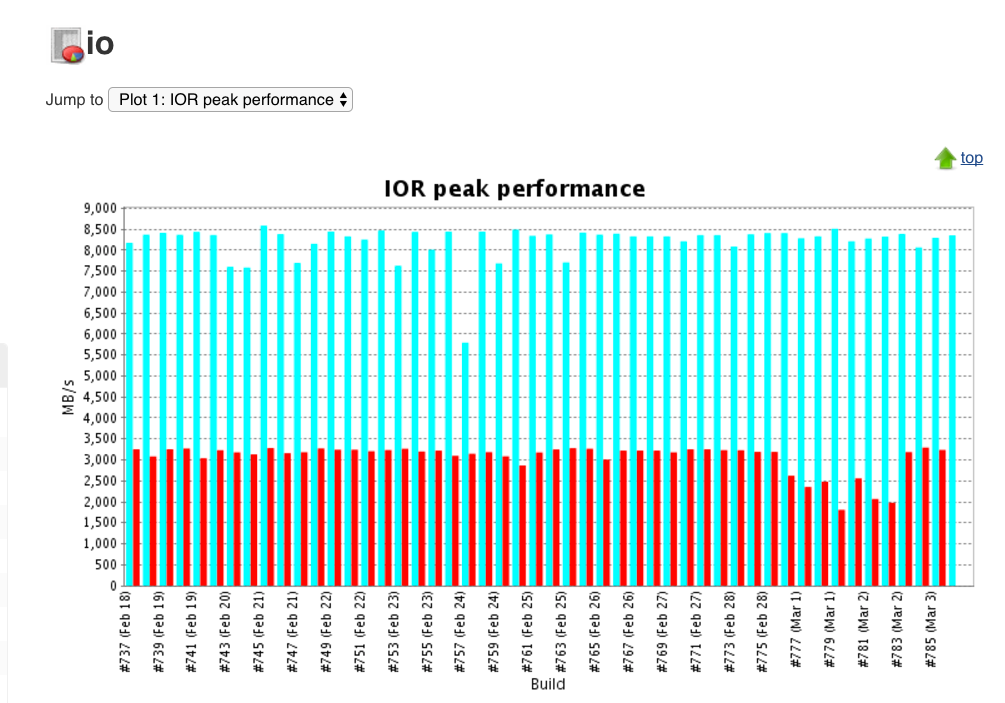
\includegraphics[width=0.5\textwidth]{IOR-plot}
\caption{ IOR plot view }
\label{fig:IOR-plot}
\end{figure}
A plot like this helps us with performance baselines and we can quickly react to changes in the software environment or filesystem configuration that adversely impact performance.

\subsection{mdtest Lustre tests}
The mdtest metadata test is run on the home and scratch filesystems to validate metadata server performance.  The IOR and mdtest user-facing tests complement the fine-grained detail we are able to glean from the backed system-side counters in our OVIS database where we record details about individual server metrics and network traffic on the Cray Gemini fabric.  
\begin{figure}[H]
\centering
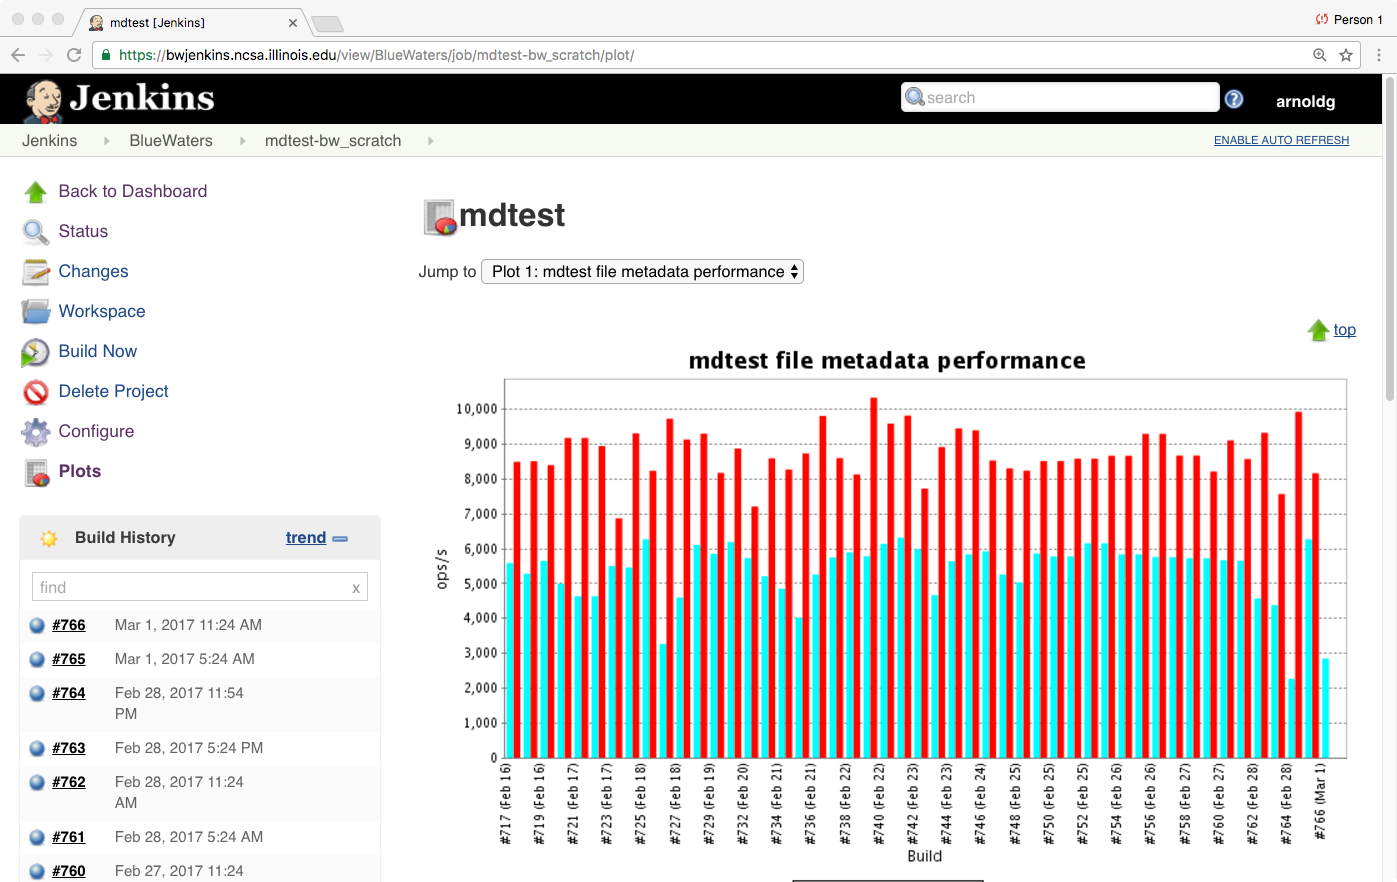
\includegraphics[width=0.5\textwidth]{mdtest-plot}
\caption{ mdtest plot view }
\label{fig:mdtest-plot}
\end{figure}

An additional best practice is to enable E-mail Notifications to the test author and/or other interested parties.  Setting notifications for unstable builds will trigger an E-mail every time the test state changes (from successful to failing and once again when successful ).
\begin{figure}[H]
\centering
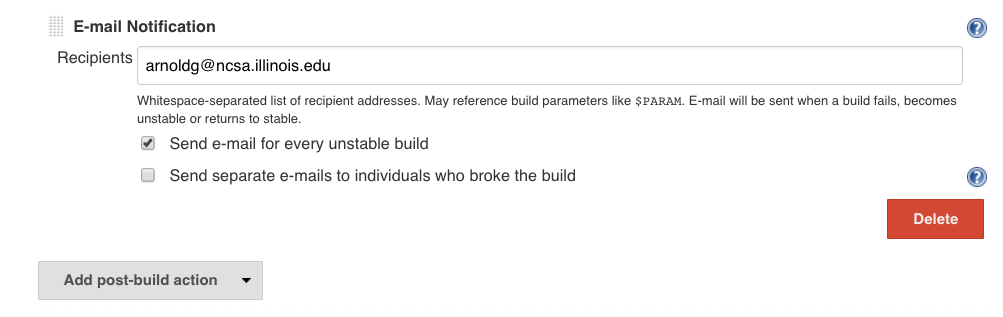
\includegraphics[width=0.5\textwidth]{mdtest-config-email}
\caption{ mdtest email configuration }
\label{fig:mdtest-config-email}
\end{figure}

\subsection{filesystem dashboard}
Our Jenkins instance is a source of information for a filesystem dashboard display we maintain in our wiki.  The "http://" urls for the plot images are shown on the dashboard and provide a recent-time display of filesystem metrics from a user point of view.  We add a Jenkins test to track response time of /bin/ls on the login nodes--a reasonable metric of metadata server health and also the most common problem reported by users when we are having filesystem issues.
\begin{figure}[H]
\centering
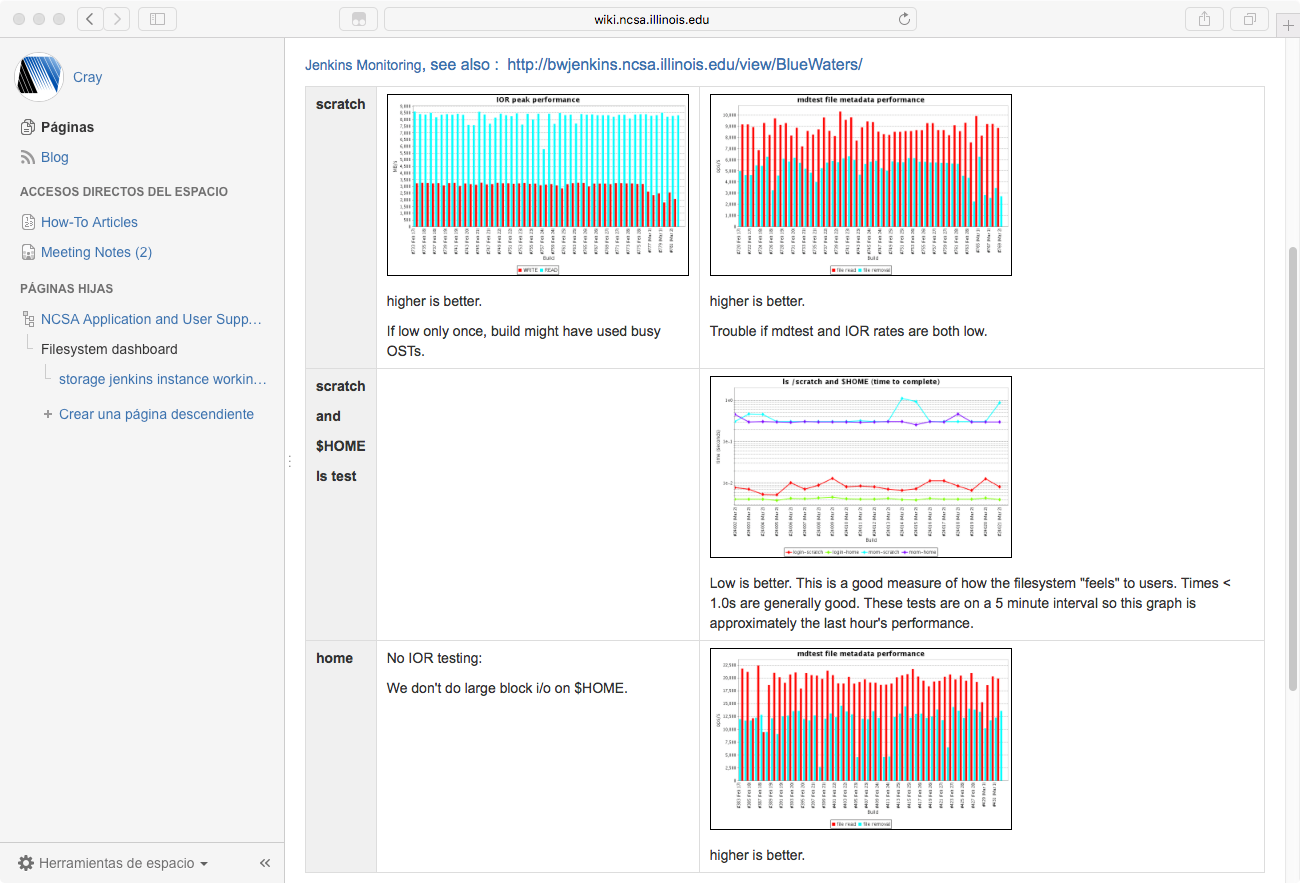
\includegraphics[width=0.5\textwidth]{wiki-dashboard}
\caption{ filesystem dashboard displaying multiple Jenkins plots }
\label{fig:wiki-dashboard}
\end{figure}

\subsection{special projects}
The initial display tabs in our Jenkins instance are used to group tests and we add tabs for special projects.   For example we clone existing tests for evaluating a new software stack on our test login node.   Our test rack has a separate set of tests from our production system and is used as our Jenkins development mule.  The sustained petascale performance benchmarks are in their own tab because they run at scale and are only run on-demand by staff (not scheduled by Jenkins ).
\begin{figure}[H]
\centering
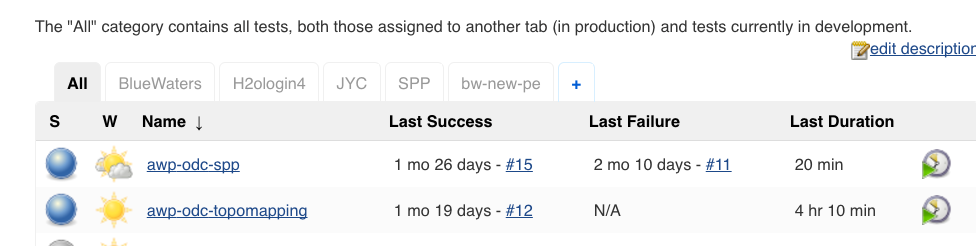
\includegraphics[width=0.5\textwidth]{tabs-display}
\caption{ tabs for project areas }
\label{fig:tabs-display}
\end{figure}

\section{Best Practices}
\begin{itemize}
\item Tests are developed on the JYC development rack and not assigned into a Jenkins tab until reviewed.
\item Email notification is enabled for most tests and the field is always populated with a test owner.
\item All tests contain a description that describes what is tested, resources required, scheduling frequency, and overall summary  to be readable by the management team.
\item Log file count is limited in the test configuration to keep from filling filesystem space with verbose logs.
\item Tests are coded to be more verbose than necessary so that failures can be isolated quickly and easily.
\end{itemize}

\section{Conclusion}
\subsection{reproducibility and regression testing}
\subsection{rapid reaction}
\subsection{caveats}
Transient errors with Jenkins sometimes occur--particularly with the Jenkins ssh subsystem.  It's not unusual to get failure rates of 1/100 from an ssh failure which is completely transient (immediately running the test again manually clears the issue on the dashboard).
\label{sec:conclusion}

% use section* for acknowledgement
\section*{Acknowledgment}
This research used resources at the National Institute for Computational Sciences, funded by the National Science Foundation (NSF).

% trigger a \newpage just before the given reference
% number - used to balance the columns on the last page
% adjust value as needed - may need to be readjusted if
% the document is modified later
\IEEEtriggeratref{8}
% The "triggered" command can be changed if desired:
\IEEEtriggercmd{\enlargethispage{-2in}}

% references section
\section*{References}
[1] http://inca.sdsc.edu/ Inca Monitoring: periodic, automated, user-level cyberinfrastructure testing
[2] https://jenkins.io/ Jenkins: open source automation server written in Java

% can use a bibliography generated by BibTeX as a .bbl file
% BibTeX documentation can be easily obtained at:
% http://www.ctan.org/tex-archive/biblio/bibtex/contrib/doc/
% The IEEEtran BibTeX style support page is at:
% http://www.michaelshell.org/tex/ieeetran/bibtex/
%\bibliographystyle{IEEEtran}
% argument is your BibTeX string definitions and bibliography database(s)
%\bibliography{IEEEabrv,../bib/paper}
%
% <OR> manually copy in the resultant .bbl file
% set second argument of \begin to the number of references
% (used to reserve space for the reference number labels box)

%\begin{thebibliography}{9}

%\bibliographystyle{IEEEtran}
%\bibliographystyle{unsrt}
%\bibliography{references}

%\end{thebibliography}

% that's all folks
\end{document}
